\documentclass[12pt]{article}

\usepackage{amsmath, mathtools}
\usepackage{amsfonts}
\usepackage{amssymb}
\usepackage{graphicx}
\usepackage{colortbl}
\usepackage{xr}
\usepackage{hyperref}
\usepackage{longtable}
\usepackage{xfrac}
\usepackage{tabularx}
\usepackage{float}
\usepackage{siunitx}
\usepackage{booktabs}
\usepackage{caption}
\usepackage{pdflscape}
\usepackage{afterpage}

\usepackage[round]{natbib}

\usepackage{titlesec}

%\usepackage{refcheck}

\hypersetup{
    bookmarks=true,         % show bookmarks bar?
      colorlinks=true,       % false: boxed links; true: colored links
    linkcolor=red,          % color of internal links (change box color with linkbordercolor)
    citecolor=green,        % color of links to bibliography
    filecolor=magenta,      % color of file links
    urlcolor=cyan           % color of external links
}

%% Comments
\usepackage{color}
\newif\ifcomments\commentstrue %displays comments
%\newif\ifcomments\commentsfalse %so that comments do not display
\ifcomments
\newcommand{\authornote}[3]{\textcolor{#1}{[#3 ---#2]}}
\newcommand{\todo}[1]{\textcolor{red}{[TODO: #1]}}
\else
\newcommand{\authornote}[3]{}
\newcommand{\todo}[1]{}
\fi
\newcommand{\wss}[1]{\authornote{blue}{SS}{#1}} 
\newcommand{\plt}[1]{\authornote{magenta}{TPLT}{#1}} %For explanation of the template
\newcommand{\an}[1]{\authornote{cyan}{Author}{#1}}
%% Common Parts
\newcommand{\progname}{4TB6 - Mechatronics Capstone} % PUT YOUR PROGRAM NAME HERE
\newcommand{\authname}{Team \#5, Locked \& Loaded
\\ Abi Nevo, nevoa
\\ Elsa Bassi, bassie
\\ Steffi Ralph, ralphs1
\\ Abdul Iqbal, iqbala18
\\ Stephen De Jong, dejons1
\\ Anthony Shenouda, shenoa2} % AUTHOR NAMES                  

\usepackage{hyperref}
    \hypersetup{colorlinks=true, linkcolor=blue, citecolor=blue, filecolor=blue,
                urlcolor=blue, unicode=false}
    \urlstyle{same}


% For easy change of table widths
\newcommand{\colZwidth}{1.0\textwidth}
\newcommand{\colAwidth}{0.13\textwidth}
\newcommand{\colBwidth}{0.82\textwidth}
\newcommand{\colCwidth}{0.1\textwidth}
\newcommand{\colDwidth}{0.05\textwidth}
\newcommand{\colEwidth}{0.8\textwidth}
\newcommand{\colFwidth}{0.17\textwidth}
\newcommand{\colGwidth}{0.5\textwidth}
\newcommand{\colHwidth}{0.28\textwidth}

% Used so that cross-references have a meaningful prefix
\newcounter{defnum} %Definition Number
\newcommand{\dthedefnum}{GD\thedefnum}
\newcommand{\dref}[1]{GD\ref{#1}}
\newcounter{datadefnum} %Datadefinition Number
\newcommand{\ddthedatadefnum}{DD\thedatadefnum}
\newcommand{\ddref}[1]{DD\ref{#1}}
\newcounter{theorynum} %Theory Number
\newcommand{\tthetheorynum}{T\thetheorynum}
\newcommand{\tref}[1]{T\ref{#1}}
\newcounter{tablenum} %Table Number
\newcommand{\tbthetablenum}{T\thetablenum}
\newcommand{\tbref}[1]{TB\ref{#1}}
\newcounter{assumpnum} %Assumption Number
\newcommand{\atheassumpnum}{P\theassumpnum}
\newcommand{\aref}[1]{A\ref{#1}}
\newcounter{goalnum} %Goal Number
\newcommand{\gthegoalnum}{P\thegoalnum}
\newcommand{\gsref}[1]{GS\ref{#1}}
\newcounter{instnum} %Instance Number
\newcommand{\itheinstnum}{IM\theinstnum}
\newcommand{\iref}[1]{IM\ref{#1}}
\newcounter{reqnum} %Requirement Number
\newcommand{\rthereqnum}{P\thereqnum}
\newcommand{\rref}[1]{R\ref{#1}}
\newcounter{nfrnum} %NFR Number
\newcommand{\rthenfrnum}{NFR\thenfrnum}
\newcommand{\nfrref}[1]{NFR\ref{#1}}
\newcounter{lcnum} %Likely change number
\newcommand{\lthelcnum}{LC\thelcnum}
\newcommand{\lcref}[1]{LC\ref{#1}}

\usepackage{fullpage}

\newcommand{\deftheory}[9][Not Applicable]
{
\newpage
\noindent \rule{\textwidth}{0.5mm}

\paragraph{RefName: } \textbf{#2} \phantomsection 
\label{#2}

\paragraph{Label:} #3

\noindent \rule{\textwidth}{0.5mm}

\paragraph{Equation:}

#4

\paragraph{Description:}

#5

\paragraph{Notes:}

#6

\paragraph{Source:}

#7

\paragraph{Ref.\ By:}

#8

\paragraph{Preconditions for \hyperref[#2]{#2}:}
\label{#2_precond}

#9

\paragraph{Derivation for \hyperref[#2]{#2}:}
\label{#2_deriv}

#1

\noindent \rule{\textwidth}{0.5mm}

}

%\documentclass{article}


\setcounter{secnumdepth}{4}

\titleformat{\paragraph}
{\normalfont\normalsize\bfseries}{\theparagraph}{1em}{}
\titlespacing*{\paragraph}
{0pt}{3.25ex plus 1ex minus .2ex}{1.5ex plus .2ex}


\begin{document}

\title{Software Requirements Specification for \progname: Smart Bike Lock} 
\author{Abi Nevo\\Elsa Bassi\\Steffi Ralph\\Abdul Iqbal\\Stephen De Jong\\Anthony Shenouda}
\date{\today}
	
\maketitle

~\newpage

\pagenumbering{roman}

\tableofcontents

~\newpage

\section*{Revision History}

\begin{tabularx}{\textwidth}{p{2cm}p{2cm}p{2cm}X}
\toprule {\bf Date} & {\bf Version} & {\bf Name} & {\bf Notes}\\
\midrule
02-10-22 & 1.0 & Elsa & Drafted first draft\\
03-10-22& 1.1 & Stephen & Drafted 1 \& 5, and formating updates\\
\bottomrule
\end{tabularx}

~\newpage

\section{Reference Material}

This section records information for easy reference.

\subsection{Table of Units}

Throughout this document SI (Syst\`{e}me International d'Unit\'{e}s) is employed
as the unit system.  In addition to the basic units, several derived units are
used as described below.  For each unit, the symbol is given followed by a
description of the unit and the SI name.
~\newline

\renewcommand{\arraystretch}{1.2}
%\begin{table}[ht]
%\begincenter
  \noindent \begin{tabular}{l l l} 
    \toprule		
    \textbf{symbol} & \textbf{unit} & \textbf{SI}\\
    \midrule 
    \si{\metre} & length & metre\\
    \si{\kilogram} & mass	& kilogram\\
    \si{\second} & time & second\\
    \si{\joule} & energy & joule\\
    P or \si{\watt} & power & watt (W = \si{\joule\per\second})\\
    \si{\ampere} or I& current & ampere\\
    \si{\ohm} or R& resistance & ohm\\
    \si{\volt} & voltage & volt\\
    \si{\newton} & force & newton\\
    \si{\newton}M & torque & newton meter\\
    \bottomrule
  \end{tabular}
  %	\caption{Provide a caption}
%\end{table}

\subsection{Table of Symbols}

The table that follows summarizes the symbols used in this document along with
their units.  The choice of symbols was made to be consistent with the heat
transfer literature and with existing documentation for solar water heating
systems.  The symbols are listed in alphabetical order.

\renewcommand{\arraystretch}{1.2}
%\noindent \begin{tabularx}{1.0\textwidth}{l l X}
\noindent \begin{longtable*}{l l p{12cm}} \toprule
\textbf{symbol} & \textbf{unit} & \textbf{description}\\
\midrule 
$B_L$ & hour & battery lifein hours\\
$B_C$ & mAH & battery capacity in amp hours\\
$L_C$ & A/actuation & current drawn per motor actuation\\
$A_\text{num}$ & actuation/charge & number of actuations per charge\\ 
\bottomrule
\end{longtable*}


\subsection{Abbreviations and Acronyms}

\renewcommand{\arraystretch}{1.2}
\begin{tabular}{l l} 
  \toprule		
  \textbf{symbol} & \textbf{description}\\
  \midrule 
  SRS & Software Requirements Specification\\
  \bottomrule
\end{tabular}\\


%\subsection{Mathematical Notation}

\pagenumbering{arabic}


\section{Introduction}

The purpose of the Smart Lock project is to design and build a product that will provide bicycle users with a safer, easier, and more accessible way to secure their bike through their smartphone. Additionally, it will provide users with a GPS feature to locate the lock in case of bike theft or misplacement.  It will consist of a physical lock that mounts to a bike and a smartphone application that will function as the user interface through which the lock can be engaged and disengaged wirelessly, as well as located. The project will provide an engineering solution using wireless communication, mechanical design, and smartphone application development. More broadly, it seeks to encourage members of society to pursue biking, in both a transportation and recreational capacity, improving the health of society’s citizens and its environment.  

\subsection{Purpose of Document}

The Requirements Documentation seeks to provide a complete overview of the requirements of the Smart Lock system so as to define the project. The assumptions, inputs and outputs will also be defined in order to outline the problem. Several models will be developed and lastly, likely and unlikely changes will be described. This will communicate a unified and documented plan for the project that can be used after the design stage to verify its functionality and provide an important benchmark. 

\subsection{Scope of Requirements} 

The Smart Lock project will build off existing designs to tie together principles of wireless communication, GPS, a mechanical locking mechanism, electrical actuation, and smartphone application development. The system will provide all functions necessary for effective and secure locking and location.  

The Smart Lock project will be designed to perform the following functions for the user.  

\begin{enumerate}
\item Wireless communication from the smartphone to the lock and vice versa. 
\item Display of lock and battery status information on the app. 
\item Display of GPS location on the app. 
\item Store and use a replaceable battery. 
\item House a mechanical lock frame. 
\item Perform electrical engagement/disengagement of a locking mechanism. 
\item Be waterproof. 
\end{enumerate}

Not included in the project scope will be Bluetooth wireless connective capabilities, a fully autonomous locking mechanism (one that will both open/close and engage/disengage the lock wirelessly) and a rechargeable battery. We will also be ignoring extreme weather and temperature conditions and their impact on the material properties.

\subsection{Characteristics of Intended Reader} \label{sec_IntendedReader}

The reader will have basic knowledge of how bikes are secured in public settings, namely using mechanical locks and keys or combination locks. They will understand why bike locking is necessary and what it means for a bike to be vulnerable to theft, i.e. that all main parts of the bike must be secured including the frame and wheels. They will also have basic knowledge of GPS and wireless communications that can be accessed through smartphone applications. Lastly, the reader will have a high-school level understanding of kinematic and electronics-related physics and math such that they can grasp the mechanical and electrical functionality of the system.  

\subsection{Organization of Document}

The document will follow the base template provided by the Capstone 4TB6 course GitLab. It will be organized with an increasing order of specificity, beginning with the General System Description that will include an overview of the Smart Lock project. The Specific System Description will make up the bulk of the document, describing the project in greater detail with its assumptions, inputs and outputs, goals and models. Finally, since the context of the project is previously stated, the Functional and Non-Functional Requirements will be outlined, as well as any foreseen Likely and Unlikely Changes to the project. Lastly, the Traceability Matrix is included to define the relationships between various relevant formulas, sections and information in the document and how they be used to build the project.  

\section{General System Description}

This section provides general information about the system.  It identifies the
interfaces between the system and its environment, describes the user
characteristics and lists the system constraints.  \plt{This text can likely be
  borrowed verbatim.}

\plt{The purpose of this section is to provide general information about the
  system so the specific requirements in the next section will be easier to
  understand. The general system description section is designed to be
  changeable independent of changes to the functional requirements documented in
  the specific system description. The general system description provides a
  context for a family of related models.  The general description can stay the
  same, while specific details are changed between family members.}

\subsection{System Context}

 \begin{figure}[h!]
 \begin{center}
 %\rotatebox{-90}
 {
  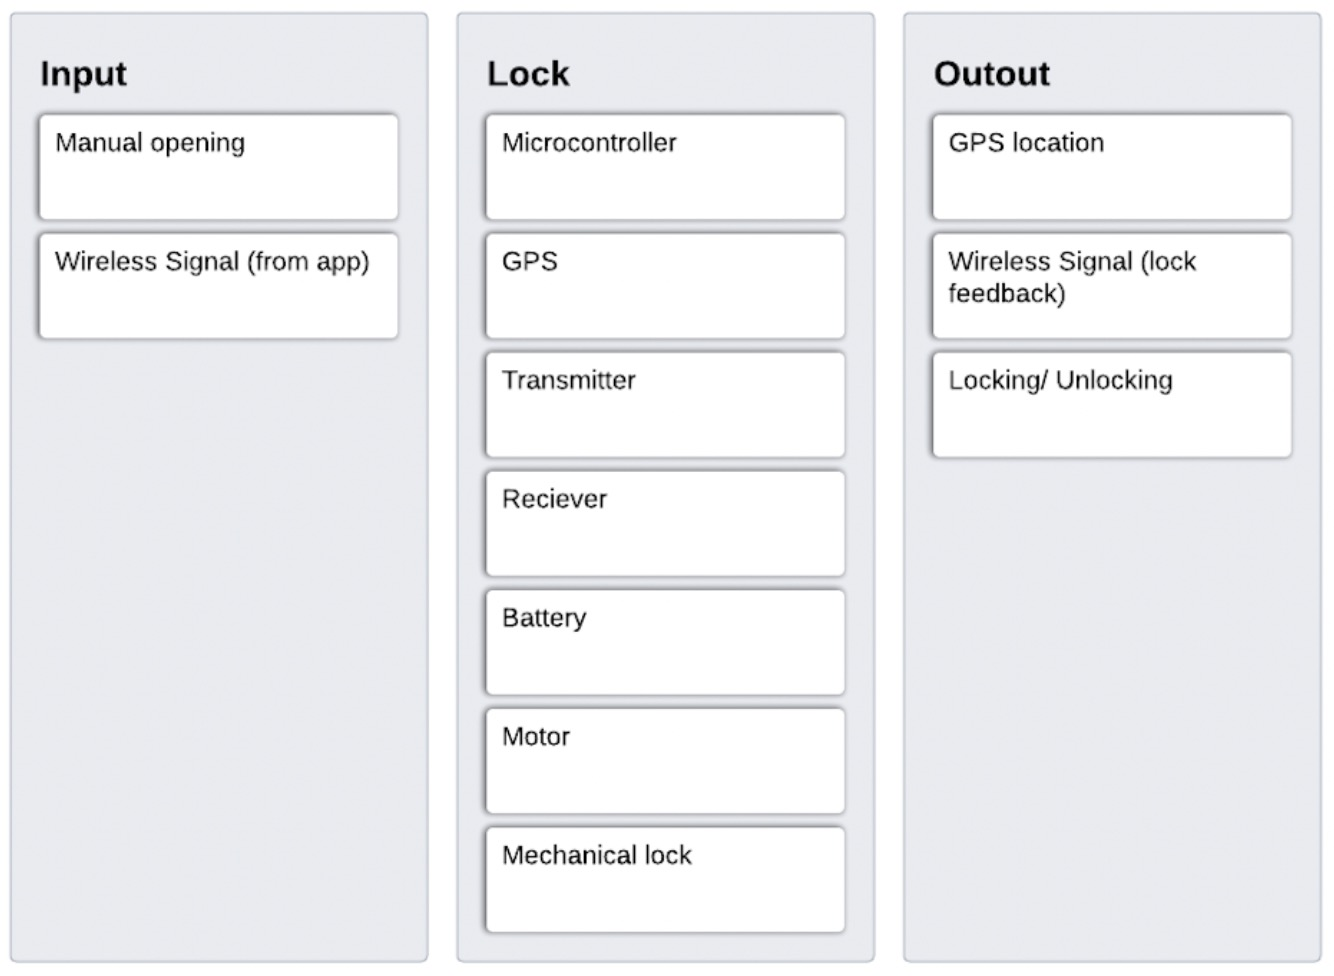
\includegraphics[width=0.6\linewidth]{../SystemContextDiagram.jpeg}
 }
 \caption{\label{The System Context}The System Context: Shows the inputs, the entities that manipulate them, and the outputs.}
 \end{center}
 \end{figure}

\begin{itemize}
\item User Responsibilities:
\begin{itemize}
\item 
\end{itemize}
\item \progname{} Responsibilities:
\begin{itemize}
\item Detect data type mismatch, such as a string of characters instead of a
  floating point number
\item 
\end{itemize}
\end{itemize}

\subsection{User Characteristics} \label{SecUserCharacteristics}

\plt{This section summarizes the knowledge/skills expected of the user.
  Measuring usability, which is often a required non-function requirement,
  requires knowledge of a typical user.  As mentioned above, the user is a
  different role from the ``intended reader,'' as given in
  Section~\ref{sec_IntendedReader}.  As in Section~\ref{sec_IntendedReader}, the
  user characteristics should be specific an unambiguous.  For instance, ``The
  end user of \progname{} should have an understanding of undergraduate Level 1
  Calculus and Physics.''}

\subsection{System Constraints}

The system has the following constraints.

\begin{itemize}

\item GPS to accurately locate the bike within a tolerance of 50 meters.
	\begin{itemize}
		\item Justification: Complex software like Google Maps ensures an accuracy of around 20 meters. Considering users only 		require the general location and our software will not be as complex as Google’s, the team added this constraint. 
	\end{itemize}
%Source: https://support.google.com/maps/answer/2839911?hl=en\&co=GENIE.Platform\%3DAndroid 

\item Total mass of lock under 3 kg. 
	\begin{itemize} 
		\item Justification: Average weight of a bike lock is just under 3 pounds. To ensure the lock was not significantly 				heavier the team added this constraint.
	\end{itemize}
%Source: https://www.nytimes.com/wirecutter/reviews/best-bike-lock/ 

\item App storage under 50 megabytes. 
	\begin{itemize} 
		\item Justification: A small mobile app should not take significant space on the user's phone. Similar GPS applications 			are around 50 megabytes.
	\end{itemize}
%Source: https://apps.apple.com/us/app/gps-fields-area-measure/id1123033235 

\item The budget for testing, designing, and equipment is \$750.
	\begin{itemize}
		\item Justification: Smart Lock has a limited budget to work within to encourage efficient use of materials and ensure low 			costs
	\end{itemize} 

\end{itemize}

\section{Specific System Description}


\subsection{Problem Description} \label{Sec_pd}

There are many problems associated with bike locks today.  People often forget or lose their keys, lock or combination.  Additionally, current locking systems are often not comprehensive – they may not lock all parts of the bike that can be stolen, namely the seat, front and back wheels, and frame.  


Furthermore, bike locks can be bulky, heavy and dangerous to carry around. It can also be tedious to find and lock one’s bike to an external frame.  The combination of these nuisances can lead to individuals leaving their bikes without properly securing them.  The city of Toronto reports an average 3625 stolen bikes annually, and the Canadian Cycling Magazine estimates that only 15-20\% of stolen bikes are reported, which indicates a rather expansive problem that can be solved [1,2].  

\subsubsection{Terminology and  Definitions}

The terms listed below will be used throughout the scope of this document and should be referenced when referring to specific components.  

\begin{itemize}
\item Smart Lock: The scope of this project and document referring to both the mechanical lock and the mobile application communicating with it. 
\item Lock: The physical component of the Smart Lock; includes the hardware, battery, motor, and locking mechanism.  
\item Team: Refers to the members working on Smart Lock 
\item App: The mobile application used to communicate with the lock 
\item Open/Close: The process of physically moving the lock frame into a state where it can be latched onto something else. 
\item Open/Close Status: The current state of the lock frame. 
\item Engage/Disengage: The automated process to actuate the lock to secure the frame. 
\item Wireless Signalling: The means of communication between the lock and the mobile application. 
\item Battery: The power source used to power the motor for engaging and disengaging. 
\item Battery Status: A measure of the quantity of charge in the battery. 
\item Git: The platform used to store the documentation and software and track changes made to the files. 
\item XCode and Flutter: The IDE used to develop the mobile application. 
\item Cross-Platform Development: The means of developing the mobile application on both iOS and Android devices. 
\item Transmitter: The device used to send signals to and from the app to give status information and to send the engagement and disengagement signals. 
\item GPS: The satellite-based navigation system used to locate the bike. 
\item Receiver: The device used to receive the signals from the app for engagement and disengagement. 
\item Microcontroller: The programmable device used to control the motor. 
\end{itemize}

\subsubsection{Physical System Description} \label{sec_phySystDescrip}

 \begin{figure}[h!]
 \begin{center}
 %\rotatebox{-90}
 {
 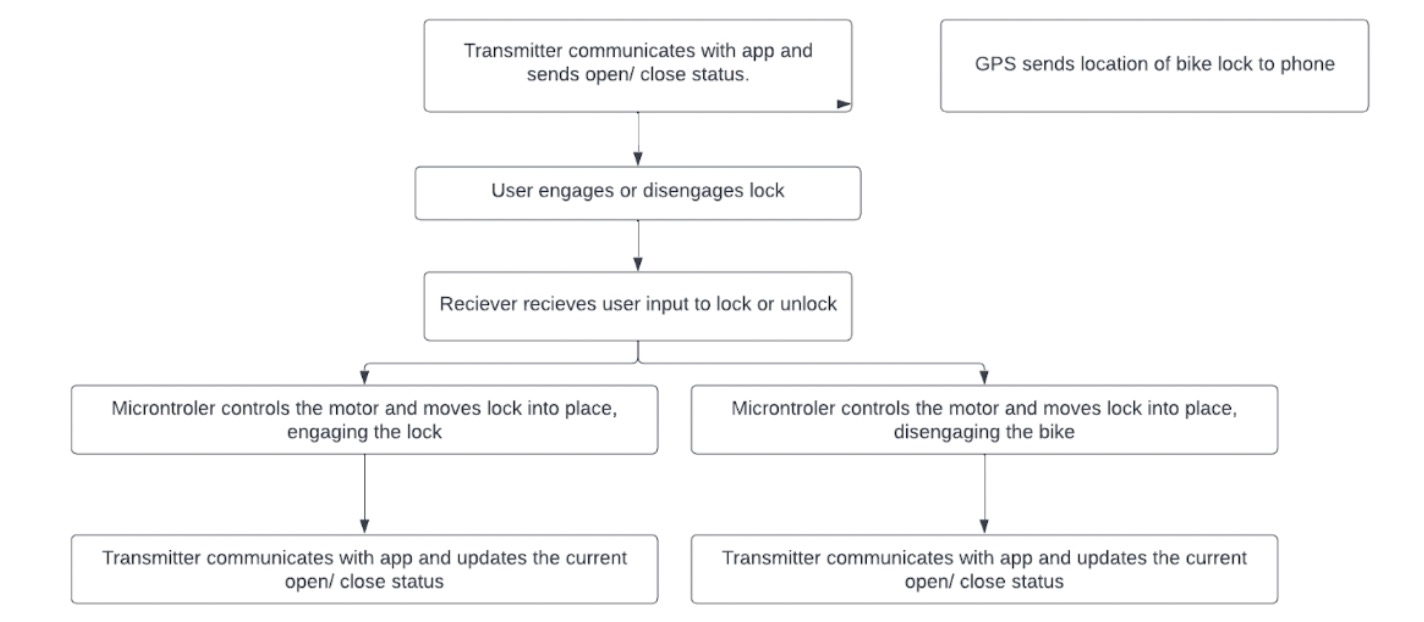
\includegraphics[width=0.6\linewidth]{../FunctionalDiagram.jpeg}
 }
 \caption{\label{The Physical System} The Physical System}
 \end{center}
 \end{figure}

\subsubsection{Goal Statements}



\noindent Given the \plt{inputs}, the goal statements are:

\begin{itemize}

\item[GS\refstepcounter{goalnum}\thegoalnum :] Effective Bike Lock: The lock is sturdy and cannot be manual opened by the average human once engaged.

\item[GS\refstepcounter{goalnum}\thegoalnum :] Long Lasting Battery Life: The power source is used efficiently to last a sufficient period of time without requiring replacement. 

\item[GS\refstepcounter{goalnum}\thegoalnum :] Bicycle Versatility: The lock can be used on mountain, city, kids, and road bikes.

\item[GS\refstepcounter{goalnum}\thegoalnum :] Easily Mountable on Bike Frame: Does not require special tools to be installed. 

\item[GS\refstepcounter{goalnum}\thegoalnum :] Effective GPS Tracking: The lock can accurately transmit location to app regardless of location.  

\item[GS\refstepcounter{goalnum}\thegoalnum :] Weatherproof: The lock is not easily damaged by wind, rain, snow, heat, and cold weather.

\end{itemize}

\subsubsection{Assumptions} \label{sec_assumpt}

\begin{itemize}

\item The bike will be left in locations with strong GPS signal.
Dependencies: Locations such as garages and underground parking. 
\item The user’s phone will always be able to connect to the lock (wireless connection works as intended).
Dependencies: All users have modern phones that can operate the application. The phones will also have functional location settings.  
\item Users will have no limiting physical disabilities.
Dependencies: Average person is strong enough to manually lock and unlock the bike.
\item The lock will be weatherproof.
Dependencies: Rain, snow or extreme temperatures will not damage the lock. 
\item Battery life is only reduced when the motor is being used.
Dependencies: Battery life is independent of weather and time.
\item Efficiency is always constant.
Dependencies: The battery's power does not decrease over time.

\end{itemize}

\subsubsection{Theoretical Models}\label{sec_theoretical}

~\newline

\noindent
\deftheory
% #2 refname of theory
% #3 label
{Torque of a Motor}
% #4 equation
{
  ${\bf T = F \cdot d} = {\bf I  \cdot  k_T}$
}

% #5 description
{
The above equation gives the torque $T$ (\si{\newton\metre}) required to actuate the opening and closing mechanism of the lock through the motor. Torque is equal to the force $F$ (\si{\newton}) to open or close the lock, multiplied by the distance $d$ (\si{\metre}) from the motor's axis of rotation. To extract current, torque is also equal to the load (motor) current $I$ (\si{\ampere}) multiplied by the motor's torque Constant $k_T$ (\si{\newton\metre\per\ampere}).  

The net force will be calculated once the design is finalized. The distance and torque constant will be dependent on the motor. These equations will be used to calculate the current required from the battery. They must be computed twice; once for engaging, and again for disengaging. 
}
% #6 Notes
{
None.
}
% #7 Source
{
  \url{https://www.motioncontroltips.com/faq-whats-the-relationship-between-current-and-dc-motor-output-torque/ }
}
% #8 Referenced by
{
  \dref{ROCT}
}
% #9 Preconditions
{
None
}
% #1 derivation - not applicable by default
{}

~\newline

\noindent
\deftheory
% #2 refname of theory
% #3 label
{Ohm's Law}
% #4 equation
{
  $V = I \cdot R$
}

% #5 description
{
The above equation gives the voltage $V$ (\si{\volt}), which is equal to the load (motor) current $I$ (\si{\ampere}) multiplied by the resistance $R$ (\si{\ohm}) of the motor. This can be used to find the rating of battery needed to power the motor. This calculation must also be done twice as outlined above.
}
% #6 Notes
{
None.
}
% #7 Source
{

}
% #8 Referenced by
{
  \dref{ROCT}
}
% #9 Preconditions
{
None
}
% #1 derivation - not applicable by default
{}

~\newline

\noindent
\deftheory
% #2 refname of theory
% #3 label
{Battery Life}
% #4 equation
{
  ${\bf BL = \frac{BC}{I}}$
}

% #5 description
{
The above equation gives the battery life $BL$ (\si{\hour}), which will be calculated by dividing the battery capacity $BC$ (\si{\ampere\hour}) selected and the load current $I$ (\si{\ampere)}.
}
% #6 Notes
{
None.
}
% #7 Source
{
 
}
% #8 Referenced by
{
  \dref{ROCT}
}
% #9 Preconditions
{
None
}
% #1 derivation - not applicable by default
{}

~\newline

\subsubsection{General Definitions}\label{sec_gendef}

\plt{General Definitions (GDs) are a refinement of one or more TMs, and/or of
  other GDs.  The GDs are less abstract than the TMs.  Generally the reduction
  in abstraction is possible through invoking (using/referencing) Assumptions.
  For instance, the TM could be Newton's Law of Cooling stated abstracting.  The
  GD could take the general law and apply it to get a 1D equation.}

This section collects the laws and equations that will be used in building the
instance models.

\plt{Some projects may not have any content for this section, but the section
  heading should be kept.}  \plt{Modify the examples below for your problem, and
  add additional definitions as appropriate.}

~\newline

\noindent
\begin{minipage}{\textwidth}
\renewcommand*{\arraystretch}{1.5}
\begin{tabular}{| p{\colAwidth} | p{\colBwidth}|}
\hline
\rowcolor[gray]{0.9}
Number& GD\refstepcounter{defnum}\thedefnum \label{NL}\\
\hline
Label &\bf Newton's law of cooling \\
\hline
% Units&$MLt^{-3}T^0$\\
% \hline
SI Units&\si{\watt\per\square\metre}\\
\hline
Equation&$ q(t) = h \Delta T(t)$  \\
\hline
Description &
Newton's law of cooling describes convective cooling from a surface.  The law is
stated as: the rate of heat loss from a body is proportional to the difference
in temperatures between the body and its surroundings.
\\
& $q(t)$ is the thermal flux (\si{\watt\per\square\metre}).\\
& $h$ is the heat transfer coefficient, assumed independent of $T$ (\aref{A_hcoeff})
	(\si{\watt\per\square\metre\per\celsius}).\\
&$\Delta T(t)$= $T(t) - T_{\text{env}}(t)$ is the time-dependent thermal gradient
between the environment and the object (\si{\celsius}).
\\
\hline
  Source & Citation here \\
  \hline
  Ref.\ By & \ddref{FluxCoil}, \ddref{FluxPCM}\\
  \hline
\end{tabular}
\end{minipage}\\

\subsubsection*{Detailed derivation of simplified rate of change of temperature}

\plt{This may be necessary when the necessary information does not fit in the
  description field.}
\plt{Derivations are important for justifying a given GD.  You want it to be
  clear where the equation came from.}

\subsubsection{Data Definitions}\label{sec_datadef}

\plt{The Data Definitions are definitions of symbols and equations that are
  given for the problem.  They are not derived; they are simply used by other
  models.  For instance, if a problem depends on density, there may be a data
  definition for the equation defining density.  The DDs are given information
  that you can use in your other modules.}

\plt{All Data Definitions should be used (referenced) by at least one other
  model.}

This section collects and defines all the data needed to build the instance
models. The dimension of each quantity is also given.  \plt{Modify the examples
  below for your problem, and add additional definitions as appropriate.}

~\newline

\noindent
\begin{minipage}{\textwidth}
\renewcommand*{\arraystretch}{1.5}
\begin{tabular}{| p{\colAwidth} | p{\colBwidth}|}
\hline
\rowcolor[gray]{0.9}
Number& DD\refstepcounter{datadefnum}\thedatadefnum \label{FluxCoil}\\
\hline
Label& \bf Heat flux out of coil\\
\hline
Symbol &$q_C$\\
\hline
% Units& $Mt^{-3}$\\
% \hline
  SI Units & \si{\watt\per\square\metre}\\
  \hline
  Equation&$q_C(t) = h_C (T_C - T_W(t))$, over area $A_C$\\
  \hline
  Description & 
                $T_C$ is the temperature of the coil (\si{\celsius}).  $T_W$ is the temperature of the water (\si{\celsius}).  
                The heat flux out of the coil, $q_C$ (\si{\watt\per\square\metre}), is found by
                assuming that Newton's Law 
                of Cooling applies (\aref{A_Newt_coil}).  This law (\dref{NL}) is used on the surface of
                the coil, which has area $A_C$ (\si{\square\metre}) and heat 
                transfer coefficient $h_C$
                (\si{\watt\per\square\metre\per\celsius}).  This equation
                assumes that the temperature of the coil is constant over time (\aref{A_tcoil}) and that it does not vary along the length
                of the coil (\aref{A_tlcoil}).
  \\
  \hline
  Sources& Citation here \\
  \hline
  Ref.\ By & \iref{ewat}\\
  \hline
\end{tabular}
\end{minipage}\\

\subsubsection{Data Types}\label{sec_datatypes}

\plt{This section is optional.  In many scientific computing programs it isn't
  necessary, since the inputs and outpus are straightforward types, like reals,
  integers, and sequences of reals and integers.  However, for some problems it
  is very helpful to capture the type information.}

\plt{The data types are not derived; they are simply stated and used by other
  models.}

\plt{All data types must be used by at least one of the models.}

\plt{For the mathematical notation for expressing types, the recommendation is
  to use the notation of~\citet{HoffmanAndStrooper1995}.}

This section collects and defines all the data types needed to document the
models. \plt{Modify the examples below for your problem, and add additional
  definitions as appropriate.}

~\newline

\noindent
\begin{minipage}{\textwidth}
\renewcommand*{\arraystretch}{1.5}
\begin{tabular}{| p{\colAwidth} | p{\colBwidth}|}
  \hline
  \rowcolor[gray]{0.9}
  Type Name & Name for Type\\
  \hline
  Type Def & mathematical definition of the type\\
  \hline
  Description & description here
  \\
  \hline
  Sources & Citation here, if the type is borrowed from another source\\
  \hline
\end{tabular}
\end{minipage}\\

\subsubsection{Instance Models} \label{sec_instance}    

\plt{The motivation for this section is to reduce the problem defined in
  ``Physical System Description'' (Section~\ref{sec_phySystDescrip}) to one
  expressed in mathematical terms. The IMs are built by refining the TMs and/or
  GDs.  This section should remain abstract.  The SRS should specify the
  requirements without considering the implementation.}

This section transforms the problem defined in Section~\ref{Sec_pd} into 
one which is expressed in mathematical terms. It uses concrete symbols defined 
in Section~\ref{sec_datadef} to replace the abstract symbols in the models 
identified in Sections~\ref{sec_theoretical} and~\ref{sec_gendef}.

The goals \plt{reference your goals} are solved by \plt{reference your instance
  models}.  \plt{other details, with cross-references where appropriate.}
\plt{Modify the examples below for your problem, and add additional models as
  appropriate.}

~\newline

%Instance Model 1

\noindent
\begin{minipage}{\textwidth}
\renewcommand*{\arraystretch}{1.5}
\begin{tabular}{| p{\colAwidth} | p{\colBwidth}|}
  \hline
  \rowcolor[gray]{0.9}
  Number& IM\refstepcounter{instnum}\theinstnum \label{ewat}\\
  \hline
  Label& \bf Energy balance on water to find $T_W$\\
  \hline
  Input&$m_W$, $C_W$, $h_C$, $A_C$, $h_P$, $A_P$, $t_\text{final}$, $T_C$, 
  $T_\text{init}$, $T_P(t)$ from \iref{epcm}\\
  & The input is constrained so that $T_\text{init} \leq T_C$ (\aref{A_charge})\\
  \hline
  Output&$T_W(t)$, $0\leq t \leq t_\text{final}$, such that\\
  &$\frac{dT_W}{dt} = \frac{1}{\tau_W}[(T_C - T_W(t)) + {\eta}(T_P(t) - T_W(t))]$,\\
  &$T_W(0) = T_P(0) = T_\text{init}$ (\aref{A_InitTemp}) and $T_P(t)$ from \iref{epcm} \\
  \hline
  Description&$T_W$ is the water temperature (\si{\celsius}).\\
  &$T_P$ is the PCM temperature (\si{\celsius}).\\
  &$T_C$ is the coil temperature (\si{\celsius}).\\
  &$\tau_W = \frac{m_W C_W}{h_C A_C}$ is a constant (\si{\second}).\\
  &$\eta = \frac{h_P A_P}{h_C A_C}$ is a constant (dimensionless).\\
  & The above equation applies as long as the water is in liquid form,
  $0<T_W<100^o\text{C}$, where $0^o\text{C}$ and $100^o\text{C}$ are the melting
  and boiling points of water, respectively (\aref{A_OpRange}, \aref{A_Pressure}).
  \\
  \hline
  Sources& Citation here \\
  \hline
  Ref.\ By & \iref{epcm}\\
  \hline
\end{tabular}
\end{minipage}\\

%~\newline

\subsubsection*{Derivation of ...}

\plt{The derivation shows how the IM is derived from the TMs/GDs.  In cases
  where the derivation cannot be described under the Description field, it will
  be necessary to include this subsection.}

\subsubsection{Input Data Constraints} \label{sec_DataConstraints}    

Table~\ref{TblInputVar} shows the data constraints on the input output
variables.  The column for physical constraints gives the physical limitations
on the range of values that can be taken by the variable.  The column for
software constraints restricts the range of inputs to reasonable values.  The
software constraints will be helpful in the design stage for picking suitable
algorithms.  The constraints are conservative, to give the user of the model the
flexibility to experiment with unusual situations.  The column of typical values
is intended to provide a feel for a common scenario.  The uncertainty column
provides an estimate of the confidence with which the physical quantities can be
measured.  This information would be part of the input if one were performing an
uncertainty quantification exercise.

The specification parameters in Table~\ref{TblInputVar} are listed in
Table~\ref{TblSpecParams}.

\begin{table}[!h]
  \caption{Input Variables} \label{TblInputVar}
  \renewcommand{\arraystretch}{1.2}
\noindent \begin{longtable*}{l l l l c} 
  \toprule
  \textbf{Var} & \textbf{Physical Constraints} & \textbf{Software Constraints} &
                             \textbf{Typical Value} & \textbf{Uncertainty}\\
  \midrule 
  $L$ & $L > 0$ & $L_{\text{min}} \leq L \leq L_{\text{max}}$ & 1.5 \si[per-mode=symbol] {\metre} & 10\%
  \\
  \bottomrule
\end{longtable*}
\end{table}

\noindent 
\begin{description}
\item[(*)] \plt{you might need to add some notes or clarifications}
\end{description}

\begin{table}[!h]
\caption{Specification Parameter Values} \label{TblSpecParams}
\renewcommand{\arraystretch}{1.2}
\noindent \begin{longtable*}{l l} 
  \toprule
  \textbf{Var} & \textbf{Value} \\
  \midrule 
  $L_\text{min}$ & 0.1 \si{\metre}\\
  \bottomrule
\end{longtable*}
\end{table}

\subsubsection{Properties of a Correct Solution} \label{sec_CorrectSolution}

\noindent
A correct solution must exhibit \plt{fill in the details}.  \plt{These
  properties are in addition to the stated requirements.  There is no need to
  repeat the requirements here.  These additional properties may not exist for
  every problem.  Examples include conservation laws (like conservation of
  energy or mass) and known constraints on outputs, which are usually summarized
  in tabular form.  A sample table is shown in Table~\ref{TblOutputVar}}

\begin{table}[!h]
\caption{Output Variables} \label{TblOutputVar}
\renewcommand{\arraystretch}{1.2}
\noindent \begin{longtable*}{l l} 
  \toprule
  \textbf{Var} & \textbf{Physical Constraints} \\
  \midrule 
  $T_W$ & $T_\text{init} \leq T_W \leq T_C$ (by~\aref{A_charge})
  \\
  \bottomrule
\end{longtable*}
\end{table}

\plt{This section is not for test cases or techniques for verification and
  validation.  Those topics will be addressed in the Verification and Validation
  plan.}

\section{Requirements}

This section provides the functional requirements, the business tasks that the
software is expected to complete, and the nonfunctional requirements, the
qualities that the software is expected to exhibit.

\subsection{Functional Requirements}

\subsubsection{User Input Related}

\paragraph{LockButton input must engage the lock on the bike.}
\paragraph{UnlockButton input must disengage the lock on the bike }
\paragraph{When lock is engaged, change lock status to locked }
\paragraph{When lock is unengaged, change lock status to unlocked }
\paragraph{Moving locking bar closed must move OpenClosedstatus to Closed }
\paragraph{Moving locking bar open must move OpenClosedstatus to open }
\paragraph{Location (coordinates) of user’s phone must be shown on app as UserPosition }

\subsubsection{Bike Input Related}
\paragraph{The lock can be mounted to the bikes frame}

\subsubsection{Output Related}
\paragraph{Battery percentage must be shown on phone app }
\paragraph{Location (coordinates) of bike must be shown on app as BikePosition }
\paragraph{Battery must output enough power to engage/disengage the lock }


\subsection{Nonfunctional Requirements}

\subsubsection{Smart Phone}
\paragraph{can be used by people speaking different languages }
\paragraph{Can reasonably be used without requiring an instruction manual}

\subsubsection{Physical Design}
\paragraph{The design must be visual appealing }
\paragraph{The design must not impede normal bike functions}
\paragraph{The lock must be waterproofed to withstand normal rainfall}
\paragraph{The lock must be waterproofed to withstand normal splashing while riding}

\subsubsection{Accuracy}
\paragraph{Accuracy of bike lock status must be above 90\% }
\paragraph{The accuracy of gps positioning must be accurate within 10M }
\paragraph{Battery percentage must be calculated accurately within 10\% }

\subsubsection{Usability}
\paragraph{iPhone app locking must be quicker to use than a typical keyed/combo bike lock }
\paragraph{Opening and closing lock must require similar force to a typical keyed/combo }
\paragraph{Battery must last for greater than 1 month and/or 60 rides }

\subsubsection{Maintainability}
\paragraph{Should take less than X\_FRACTION of total development time }
\paragraph{Making changes to the GUI }
\paragraph{Motor/Battery Controller Software }
\paragraph{Electrical Circuit }
\paragraph{Mechanical physical design }

\subsubsection{Portability}
\paragraph{The app should run on iOS }
\paragraph{The app should be easily maintained through iOS updates }

\subsubsection{Security}
\paragraph{Lock must only be engaged/disengaged by the intended user(s) (I.e., not everyone with the app can engage/disengage the lock)}


\section{Likely Changes}    

\noindent \begin{itemize}

\item[LC\refstepcounter{lcnum}\thelcnum\label{LC_meaningfulLabel}:] \plt{Give
    the likely changes, with a reference to the related assumption (aref), as appropriate.}

\end{itemize}

\section{Unlikely Changes}    

\noindent \begin{itemize}

\item[LC\refstepcounter{lcnum}\thelcnum\label{LC_meaningfulLabel}:] \plt{Give
    the unlikely changes.  The design can assume that the changes listed will
    not occur.}

\end{itemize}

\section{Traceability Matrices and Graphs}

The purpose of the traceability matrices is to provide easy references on what
has to be additionally modified if a certain component is changed.  Every time a
component is changed, the items in the column of that component that are marked
with an ``X'' may have to be modified as well.  Table~\ref{Table:trace} shows the
dependencies of theoretical models, general definitions, data definitions, and
instance models with each other. Table~\ref{Table:R_trace} shows the
dependencies of instance models, requirements, and data constraints on each
other. Table~\ref{Table:A_trace} shows the dependencies of theoretical models,
general definitions, data definitions, instance models, and likely changes on
the assumptions.

\plt{You will have to modify these tables for your problem.}

\plt{The traceability matrix is not generally symmetric.  If GD1 uses A1, that
  means that GD1's derivation or presentation requires invocation of A1.  A1
  does not use GD1.  A1 is ``used by'' GD1.}

\plt{The traceability matrix is challenging to maintain manually.  Please do
  your best.  In the future tools (like Drasil) will make this much easier.}

\afterpage{
\begin{landscape}
\begin{table}[h!]
\centering
\begin{tabular}{|c|c|c|c|c|c|c|c|c|c|c|c|c|c|c|c|c|c|c|c|}
\hline
	& \aref{A_OnlyThermalEnergy}& \aref{A_hcoeff}& \aref{A_mixed}& \aref{A_tpcm}& \aref{A_const_density}& \aref{A_const_C}& \aref{A_Newt_coil}& \aref{A_tcoil}& \aref{A_tlcoil}& \aref{A_Newt_pcm}& \aref{A_charge}& \aref{A_InitTemp}& \aref{A_OpRangePCM}& \aref{A_OpRange}& \aref{A_htank}& \aref{A_int_heat}& \aref{A_vpcm}& \aref{A_PCM_state}& \aref{A_Pressure} \\
\hline
\tref{T_COE}        & X& & & & & & & & & & & & & & & & & & \\ \hline
\tref{T_SHE}        & & & & & & & & & & & & & & & & & & & \\ \hline
\tref{T_LHE}        & & & & & & & & & & & & & & & & & & & \\ \hline
\dref{NL}           & & X& & & & & & & & & & & & & & & & & \\ \hline
\dref{ROCT}         & & & X& X& X& X& & & & & & & & & & & & & \\ \hline
\ddref{FluxCoil}    & & & & & & & X& X& X& & & & & & & & & & \\ \hline
\ddref{FluxPCM}     & & & X& X& & & & & & X& & & & & & & & & \\ \hline
\ddref{D_HOF}       & & & & & & & & & & & & & & & & & & & \\ \hline
\ddref{D_MF}        & & & & & & & & & & & & & & & & & & & \\ \hline
\iref{ewat}         & & & & & & & & & & & X& X& & X& X& X& & & X \\ \hline
\iref{epcm}         & & & & & & & & & & & & X& X& & & X& X& X& \\ \hline
\iref{I_HWAT}       & & & & & & & & & & & & & & X& & & & & X \\ \hline
\iref{I_HPCM}       & & & & & & & & & & & & & X& & & & & X & \\ \hline
\lcref{LC_tpcm}     & & & & X& & & & & & & & & & & & & & & \\ \hline
\lcref{LC_tcoil}    & & & & & & & & X& & & & & & & & & & & \\ \hline
\lcref{LC_tlcoil}   & & & & & & & & & X& & & & & & & & & & \\ \hline
\lcref{LC_charge}   & & & & & & & & & & & X& & & & & & & & \\ \hline
\lcref{LC_InitTemp} & & & & & & & & & & & & X& & & & & & & \\ \hline
\lcref{LC_htank}    & & & & & & & & & & & & & & & X& & & & \\
\hline
\end{tabular}
\caption{Traceability Matrix Showing the Connections Between Assumptions and Other Items}
\label{Table:A_trace}
\end{table}
\end{landscape}
}

\begin{table}[h!]
\centering
\begin{tabular}{|c|c|c|c|c|c|c|c|c|c|c|c|c|c|c|c|c|c|c|c|c|c|c|c|}
\hline        
	& \tref{T_COE}& \tref{T_SHE}& \tref{T_LHE}& \dref{NL}& \dref{ROCT} & \ddref{FluxCoil}& \ddref{FluxPCM} & \ddref{D_HOF}& \ddref{D_MF}& \iref{ewat}& \iref{epcm}& \iref{I_HWAT}& \iref{I_HPCM} \\
\hline
\tref{T_COE}     & & & & & & & & & & & & & \\ \hline
\tref{T_SHE}     & & & X& & & & & & & & & & \\ \hline
\tref{T_LHE}     & & & & & & & & & & & & & \\ \hline
\dref{NL}        & & & & & & & & & & & & & \\ \hline
\dref{ROCT}      & X& & & & & & & & & & & & \\ \hline
\ddref{FluxCoil} & & & & X& & & & & & & & & \\ \hline
\ddref{FluxPCM}  & & & & X& & & & & & & & & \\ \hline
\ddref{D_HOF}    & & & & & & & & & & & & & \\ \hline
\ddref{D_MF}     & & & & & & & & X& & & & & \\ \hline
\iref{ewat}      & & & & & X& X& X& & & & X& & \\ \hline
\iref{epcm}      & & & & & X& & X& & X& X& & & X \\ \hline
\iref{I_HWAT}    & & X& & & & & & & & & & & \\ \hline
\iref{I_HPCM}    & & X& X& & & & X& X& X& & X& & \\
\hline
\end{tabular}
\caption{Traceability Matrix Showing the Connections Between Items of Different Sections}
\label{Table:trace}
\end{table}

\begin{table}[h!]
\centering
\begin{tabular}{|c|c|c|c|c|c|c|c|}
\hline
	& \iref{ewat}& \iref{epcm}& \iref{I_HWAT}& \iref{I_HPCM}& \ref{sec_DataConstraints}& \rref{R_RawInputs}& \rref{R_MassInputs} \\
\hline
\iref{ewat}            & & X& & & & X& X \\ \hline
\iref{epcm}            & X& & & X& & X& X \\ \hline
\iref{I_HWAT}          & & & & & & X& X \\ \hline
\iref{I_HPCM}          & & X& & & & X& X \\ \hline
\rref{R_RawInputs}     & & & & & & & \\ \hline
\rref{R_MassInputs}    & & & & & & X& \\ \hline
\rref{R_CheckInputs}   & & & & & X& & \\ \hline
\rref{R_OutputInputs}  & X& X& & & & X& X \\ \hline
\rref{R_TempWater}     & X& & & & & & \\ \hline 
\rref{R_TempPCM}       & & X& & & & & \\ \hline
\rref{R_EnergyWater}   & & & X& & & & \\ \hline
\rref{R_EnergyPCM}     & & & & X& & & \\ \hline
\rref{R_VerifyOutput}  & & & X& X& & & \\ \hline
\rref{R_timeMeltBegin} & & X& & & & & \\ \hline
\rref{R_timeMeltEnd}   & & X& & & & & \\ 
\hline
\end{tabular}
\caption{Traceability Matrix Showing the Connections Between Requirements and Instance Models}
\label{Table:R_trace}
\end{table}

The purpose of the traceability graphs is also to provide easy references on
what has to be additionally modified if a certain component is changed.  The
arrows in the graphs represent dependencies. The component at the tail of an
arrow is depended on by the component at the head of that arrow. Therefore, if a
component is changed, the components that it points to should also be
changed. Figure~\ref{Fig_ATrace} shows the dependencies of theoretical models,
general definitions, data definitions, instance models, likely changes, and
assumptions on each other. Figure~\ref{Fig_RTrace} shows the dependencies of
instance models, requirements, and data constraints on each other.

% \begin{figure}[h!]
% 	\begin{center}
% 		%\rotatebox{-90}
% 		{
% 			\includegraphics[width=\textwidth]{ATrace.png}
% 		}
% 		\caption{\label{Fig_ATrace} Traceability Matrix Showing the Connections Between Items of Different Sections}
% 	\end{center}
% \end{figure}


% \begin{figure}[h!]
% 	\begin{center}
% 		%\rotatebox{-90}
% 		{
% 			\includegraphics[width=0.7\textwidth]{RTrace.png}
% 		}
% 		\caption{\label{Fig_RTrace} Traceability Matrix Showing the Connections Between Requirements, Instance Models, and Data Constraints}
% 	\end{center}
% \end{figure}

\section{Development Plan}

\plt{This section is optional.  It is used to explain the plan for developing
  the software.  In particular, this section gives a list of the order in which
  the requirements will be implemented.  In the context of a course  this is
  where you can indicate which requirements will be implemented as part of the
  course, and which will be ``faked'' as future work.  This section can be
  organized as a prioritized list of requirements, or it could should the
  requirements that will be implemented for ``phase 1'', ``phase 2'', etc.}

\section{Values of Auxiliary Constants}

\plt{Show the values of the symbolic parameters introduced in the report.}

\plt{The definition of the requirements will likely call for SYMBOLIC\_CONSTANTS.
Their values are defined in this section for easy maintenance.}

\plt{The value of FRACTION, for the Maintainability NFR would be given here.}

\newpage

\bibliographystyle {plainnat}
\bibliography {../../refs/References}

\newpage

\noindent \plt{The following is not part of the template, just some things to consider
  when filing in the template.}

\noindent \plt{Grammar, flow and \LaTeX advice:
\begin{itemize}
\item For Mac users \texttt{*.DS\_Store} should be in \texttt{.gitignore}
\item \LaTeX{} and formatting rules
\begin{itemize}
\item Variables are italic, everything else not, includes subscripts (link to
  document)
\begin{itemize}
\item \href{https://physics.nist.gov/cuu/pdf/typefaces.pdf}{Conventions}
\item Watch out for implied multiplication
\end{itemize}
\item Use BibTeX
\item Use cross-referencing
\end{itemize}
\item Grammar and writing rules
\begin{itemize}
\item Acronyms expanded on first usage (not just in table of acronyms)
\item ``In order to'' should be ``to''
\end{itemize}
\end{itemize}}

\noindent \plt{Advice on using the template:
\begin{itemize}
\item Difference between physical and software constraints
\item Properties of a correct solution means \emph{additional} properties, not
  a restating of the requirements (may be ``not applicable'' for your problem).
  If you have a table of output constraints, then these are properties of a
  correct solution.
\item Assumptions have to be invoked somewhere
\item ``Referenced by'' implies that there is an explicit reference
\item Think of traceability matrix, list of assumption invocations and list of
  reference by fields as automatically generatable
\item If you say the format of the output (plot, table etc), then your
  requirement could be more abstract
\end{itemize}
}

\newpage{}
\section*{Appendix --- Reflection}

The information in this section will be used to evaluate the team members on the
graduate attribute of Lifelong Learning.  Please answer the following questions:

\begin{enumerate}
  \item What knowledge and skills will the team collectively need to acquire to
  successfully complete this capstone project?  Examples of possible knowledge
  to acquire include domain specific knowledge from the domain of your
  application, or software engineering knowledge, mechatronics knowledge or
  computer science knowledge.  Skills may be related to technology, or writing,
  or presentation, or team management, etc.  You should look to identify at
  least one item for each team member.
  \item For each of the knowledge areas and skills identified in the previous
  question, what are at least two approaches to acquiring the knowledge or
  mastering the skill?  Of the identified approaches, which will each team
  member pursue, and why did they make this choice?
\end{enumerate}

\end{document}